\chapter{Electronic excitations}
\label{chap:electronic}

We now turn our attention to the other kind of excitations present in the model hamiltonian (\ref{eq:full-hamiltonian}), namely, the \textit{electronic} excitations.
These excitations are those that, in the absence of charge-lattice coupling, arise from the $H_{el}$ term (\ref{eq:electronic-part}).
Since they are not antisymmetric to the ground state, they are inactive in infrared and Raman spectroscopies but could be accessible by electronic probes such as ARPES\footnote{Angle Resolved Photo-Emission Spectroscopy}.
It should be noted however that ARPES probes the \textit{occupied} electronic states in a system but such an interpretation is difficult in our model.

Unlike $H_{ph}$, the electronic term $H_{el}$ is not infinite dimentional since it depends only on the position of the charges in the atomic sites. 
Using the labelling convention stated in (\ref{eq:basis-set}), $H_{el}$ can be expressed as the following 9x9 matrix:
%
\begin{equation}\label{eq:Hel-matrix} 
  H_{el} \doteq
  \left( 
    \begin{array}{ccccccccc} 
      U+2E_0 &\;\;t\;\;&\;\;0\;\;&\;\;t\;\;&0&\;\;0\;\;&\;\;0\;\;&\;\;0\;\;&0 \\
      t&0&t&0&t&0&0&0&0 \\
      0&t&2E_0 &0&0&t&0&0&0 \\
      t&0&0&0&t&0&t&0&0 \\
      0&t&0&t&U-2E_0 &t&0&t&0 \\
      0&0&t&0&t&0&0&0&t \\
      0&0&0&t&0&0&2E_0 &t&0 \\
      0&0&0&0&t&0&t&0&t \\
      0&0&0&0&0&t&0&t&U+2E_0  
    \end{array} 
  \right)
\end{equation}
%
This matrix is easily diagonalized to see that its first excited state has an energy of $\sim 1376$ cm$^{-1}$ above the ground state which is considerable higher than the phononic energies of 500 and 612.4 cm$^{-1}$.

Since $H_{el-ph}$ mixes electronic and phononic degrees of freedom, a change in the coupling parameter $\lambda_{ir}$ also changes the properties of these excitations.
Similar to the phononic excitations analyzed in the previous chapter these excitations do not remain eigenstates of $H_{el}$ for $\lambda_{ir}>0$ however, as discussed in section \ref{sec:classification}, in the middle coupling regime they remain mainly electronic in nature so we continue to refer them as such.

In Figure \ref{fig:electrSpectra} we show the energy of the three lowest electronic excitations as a function of $\lambda_{ir}$.
All energies show a monotonically decreasing behaviour with $\lambda_{ir}$, reminiscent of the phononic excitations in Figure \ref{fig:irSpectra} with little change in the small and strong coupling regimes but considerable change is in the middle coupling regime.
The first excitation starts at $\sim 1376$ cm$^{-1}$ for $\lambda_{ir}=0$ and converges to $\sim 1122$ cm$^{-1}$ for large $\lambda_{ir}$.
The electronic excitation with one additional infrared phonon also converges to this energy.
The presence of a Raman phonon rigidly increases the energies by $\omega_R=500$ cm$^{-1}$ for every $\lambda_{ir}$.
%
\begin{figure}[ht]
  \centering
  % GNUPLOT: LaTeX picture with Postscript
\begingroup
  \makeatletter
  \providecommand\color[2][]{%
    \GenericError{(gnuplot) \space\space\space\@spaces}{%
      Package color not loaded in conjunction with
      terminal option `colourtext'%
    }{See the gnuplot documentation for explanation.%
    }{Either use 'blacktext' in gnuplot or load the package
      color.sty in LaTeX.}%
    \renewcommand\color[2][]{}%
  }%
  \providecommand\includegraphics[2][]{%
    \GenericError{(gnuplot) \space\space\space\@spaces}{%
      Package graphicx or graphics not loaded%
    }{See the gnuplot documentation for explanation.%
    }{The gnuplot epslatex terminal needs graphicx.sty or graphics.sty.}%
    \renewcommand\includegraphics[2][]{}%
  }%
  \providecommand\rotatebox[2]{#2}%
  \@ifundefined{ifGPcolor}{%
    \newif\ifGPcolor
    \GPcolortrue
  }{}%
  \@ifundefined{ifGPblacktext}{%
    \newif\ifGPblacktext
    \GPblacktextfalse
  }{}%
  % define a \g@addto@macro without @ in the name:
  \let\gplgaddtomacro\g@addto@macro
  % define empty templates for all commands taking text:
  \gdef\gplbacktext{}%
  \gdef\gplfronttext{}%
  \makeatother
  \ifGPblacktext
    % no textcolor at all
    \def\colorrgb#1{}%
    \def\colorgray#1{}%
  \else
    % gray or color?
    \ifGPcolor
      \def\colorrgb#1{\color[rgb]{#1}}%
      \def\colorgray#1{\color[gray]{#1}}%
      \expandafter\def\csname LTw\endcsname{\color{white}}%
      \expandafter\def\csname LTb\endcsname{\color{black}}%
      \expandafter\def\csname LTa\endcsname{\color{black}}%
      \expandafter\def\csname LT0\endcsname{\color[rgb]{1,0,0}}%
      \expandafter\def\csname LT1\endcsname{\color[rgb]{0,1,0}}%
      \expandafter\def\csname LT2\endcsname{\color[rgb]{0,0,1}}%
      \expandafter\def\csname LT3\endcsname{\color[rgb]{1,0,1}}%
      \expandafter\def\csname LT4\endcsname{\color[rgb]{0,1,1}}%
      \expandafter\def\csname LT5\endcsname{\color[rgb]{1,1,0}}%
      \expandafter\def\csname LT6\endcsname{\color[rgb]{0,0,0}}%
      \expandafter\def\csname LT7\endcsname{\color[rgb]{1,0.3,0}}%
      \expandafter\def\csname LT8\endcsname{\color[rgb]{0.5,0.5,0.5}}%
    \else
      % gray
      \def\colorrgb#1{\color{black}}%
      \def\colorgray#1{\color[gray]{#1}}%
      \expandafter\def\csname LTw\endcsname{\color{white}}%
      \expandafter\def\csname LTb\endcsname{\color{black}}%
      \expandafter\def\csname LTa\endcsname{\color{black}}%
      \expandafter\def\csname LT0\endcsname{\color{black}}%
      \expandafter\def\csname LT1\endcsname{\color{black}}%
      \expandafter\def\csname LT2\endcsname{\color{black}}%
      \expandafter\def\csname LT3\endcsname{\color{black}}%
      \expandafter\def\csname LT4\endcsname{\color{black}}%
      \expandafter\def\csname LT5\endcsname{\color{black}}%
      \expandafter\def\csname LT6\endcsname{\color{black}}%
      \expandafter\def\csname LT7\endcsname{\color{black}}%
      \expandafter\def\csname LT8\endcsname{\color{black}}%
    \fi
  \fi
  \setlength{\unitlength}{0.0500bp}%
  \begin{picture}(6802.00,4534.00)%
    \gplgaddtomacro\gplbacktext{%
      \colorrgb{0.31,0.31,0.31}%
      \put(1210,751){\makebox(0,0)[r]{\strut{}\scriptsize 1000}}%
      \colorrgb{0.31,0.31,0.31}%
      \put(1210,1631){\makebox(0,0)[r]{\strut{}\scriptsize 1250}}%
      \colorrgb{0.31,0.31,0.31}%
      \put(1210,2510){\makebox(0,0)[r]{\strut{}\scriptsize 1500}}%
      \colorrgb{0.31,0.31,0.31}%
      \put(1210,3390){\makebox(0,0)[r]{\strut{}\scriptsize 1750}}%
      \colorrgb{0.31,0.31,0.31}%
      \put(1210,4269){\makebox(0,0)[r]{\strut{}\scriptsize 2000}}%
      \colorrgb{0.31,0.31,0.31}%
      \put(1389,484){\makebox(0,0){\strut{}\scriptsize 0}}%
      \colorrgb{0.31,0.31,0.31}%
      \put(1790,484){\makebox(0,0){\strut{}\scriptsize 0.02}}%
      \colorrgb{0.31,0.31,0.31}%
      \put(2192,484){\makebox(0,0){\strut{}\scriptsize 0.04}}%
      \colorrgb{0.31,0.31,0.31}%
      \put(2593,484){\makebox(0,0){\strut{}\scriptsize 0.06}}%
      \colorrgb{0.31,0.31,0.31}%
      \put(2994,484){\makebox(0,0){\strut{}\scriptsize 0.08}}%
      \colorrgb{0.31,0.31,0.31}%
      \put(3395,484){\makebox(0,0){\strut{}\scriptsize 0.1}}%
      \colorrgb{0.31,0.31,0.31}%
      \put(3797,484){\makebox(0,0){\strut{}\scriptsize 0.12}}%
      \colorrgb{0.31,0.31,0.31}%
      \put(4198,484){\makebox(0,0){\strut{}\scriptsize 0.14}}%
      \colorrgb{0.31,0.31,0.31}%
      \put(4599,484){\makebox(0,0){\strut{}\scriptsize 0.16}}%
      \colorrgb{0.31,0.31,0.31}%
      \put(5001,484){\makebox(0,0){\strut{}\scriptsize 0.18}}%
      \colorrgb{0.31,0.31,0.31}%
      \put(5402,484){\makebox(0,0){\strut{}\scriptsize 0.2}}%
      \colorrgb{0.31,0.31,0.31}%
      \put(5803,484){\makebox(0,0){\strut{}\scriptsize 0.22}}%
      \colorrgb{0.31,0.31,0.31}%
      \put(6204,484){\makebox(0,0){\strut{}\scriptsize 0.24}}%
      \csname LTb\endcsname%
      \put(176,2510){\rotatebox{-270}{\makebox(0,0){\strut{}$\omega_i$ (cm$^{-1}$)}}}%
      \put(3897,154){\makebox(0,0){\strut{}$\lambda_{ir}$ (eV)}}%
      \put(3997,3988){\makebox(0,0)[l]{\strut{}\scriptsize$\lambda_{ir}=0.1263$}}%
    }%
    \gplgaddtomacro\gplfronttext{%
    }%
    \gplbacktext
    \put(0,0){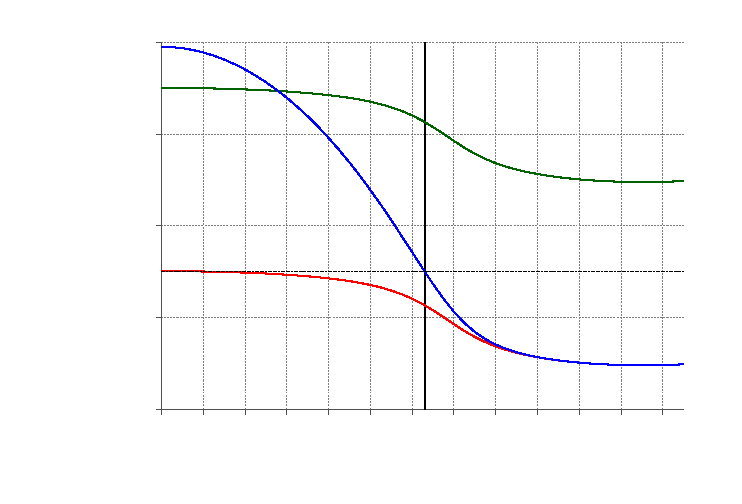
\includegraphics{images/electrSpectra}}%
    \gplfronttext
  \end{picture}%
\endgroup

  \caption[Energy of the electronic excitations as function of $\lambda_{ir}$.]
  {Energy of the electronic excitations as function of $\lambda_{ir}$. 
    The red line corresponds to an electronic excitation with zero phonons, the blue line with one infrared phonon and the green line with one Raman phonon.
    The vertical line is placed at the relevant value $\lambda_{ir}=0.1263$ eV.}
  \label{fig:electrSpectra}
\end{figure}

At $\lambda_{ir}=0.1263$ eV the first electronic excitation has the lower energy of $\sim 1282$ cm$^{-1}$ however the excitation with one additional infrared phonon has an energy of $\sim 1373$ cm$^{-1}$ which is very close to the $\sim 1376$ cm$^{-1}$ value for the first excitation at $\lambda_{ir}=0$.

\section{Partial charge localization}

We use (\ref{eq:electronOccupation}) to find the probability $P(e_1,e_2)$ of finding an excitation with the first and second charges at sites $e_1$ and $e_2$ respectively where $e_i=1,3$ denotes a charge at the oxygen sites and $e_i=2$ at the copper site.
In Figure \ref{fig:electronicOccupations} we show the probabilites for one charge in an oxygen and the other in the copper (top panel) as well as both charges in the opposing oxygen sites (bottom panel).
The probabilities of finding both charges in the same site are very low, due to the large on-site Coulumb repulsion $U=7$ eV, so we omit a figure about them.
It should be noted however that the double occupancy probabilities remain in the $\sim 0.1$\% range for the ground and first infrared excitations but are zero in the electronic excitation for all $\lambda_{ir}$.
Since the cluster is symmetric some probabilities are equivalent: $P(1,2)=P(2,1)=P(2,3)=P(3,2)$, $P(1,3)=P(3,1)$ and $P(1,1)=P(3,3)$.

\begin{figure}[ht]
  \centering
  % GNUPLOT: LaTeX picture with Postscript
\begingroup
  \makeatletter
  \providecommand\color[2][]{%
    \GenericError{(gnuplot) \space\space\space\@spaces}{%
      Package color not loaded in conjunction with
      terminal option `colourtext'%
    }{See the gnuplot documentation for explanation.%
    }{Either use 'blacktext' in gnuplot or load the package
      color.sty in LaTeX.}%
    \renewcommand\color[2][]{}%
  }%
  \providecommand\includegraphics[2][]{%
    \GenericError{(gnuplot) \space\space\space\@spaces}{%
      Package graphicx or graphics not loaded%
    }{See the gnuplot documentation for explanation.%
    }{The gnuplot epslatex terminal needs graphicx.sty or graphics.sty.}%
    \renewcommand\includegraphics[2][]{}%
  }%
  \providecommand\rotatebox[2]{#2}%
  \@ifundefined{ifGPcolor}{%
    \newif\ifGPcolor
    \GPcolortrue
  }{}%
  \@ifundefined{ifGPblacktext}{%
    \newif\ifGPblacktext
    \GPblacktextfalse
  }{}%
  % define a \g@addto@macro without @ in the name:
  \let\gplgaddtomacro\g@addto@macro
  % define empty templates for all commands taking text:
  \gdef\gplbacktext{}%
  \gdef\gplfronttext{}%
  \makeatother
  \ifGPblacktext
    % no textcolor at all
    \def\colorrgb#1{}%
    \def\colorgray#1{}%
  \else
    % gray or color?
    \ifGPcolor
      \def\colorrgb#1{\color[rgb]{#1}}%
      \def\colorgray#1{\color[gray]{#1}}%
      \expandafter\def\csname LTw\endcsname{\color{white}}%
      \expandafter\def\csname LTb\endcsname{\color{black}}%
      \expandafter\def\csname LTa\endcsname{\color{black}}%
      \expandafter\def\csname LT0\endcsname{\color[rgb]{1,0,0}}%
      \expandafter\def\csname LT1\endcsname{\color[rgb]{0,1,0}}%
      \expandafter\def\csname LT2\endcsname{\color[rgb]{0,0,1}}%
      \expandafter\def\csname LT3\endcsname{\color[rgb]{1,0,1}}%
      \expandafter\def\csname LT4\endcsname{\color[rgb]{0,1,1}}%
      \expandafter\def\csname LT5\endcsname{\color[rgb]{1,1,0}}%
      \expandafter\def\csname LT6\endcsname{\color[rgb]{0,0,0}}%
      \expandafter\def\csname LT7\endcsname{\color[rgb]{1,0.3,0}}%
      \expandafter\def\csname LT8\endcsname{\color[rgb]{0.5,0.5,0.5}}%
    \else
      % gray
      \def\colorrgb#1{\color{black}}%
      \def\colorgray#1{\color[gray]{#1}}%
      \expandafter\def\csname LTw\endcsname{\color{white}}%
      \expandafter\def\csname LTb\endcsname{\color{black}}%
      \expandafter\def\csname LTa\endcsname{\color{black}}%
      \expandafter\def\csname LT0\endcsname{\color{black}}%
      \expandafter\def\csname LT1\endcsname{\color{black}}%
      \expandafter\def\csname LT2\endcsname{\color{black}}%
      \expandafter\def\csname LT3\endcsname{\color{black}}%
      \expandafter\def\csname LT4\endcsname{\color{black}}%
      \expandafter\def\csname LT5\endcsname{\color{black}}%
      \expandafter\def\csname LT6\endcsname{\color{black}}%
      \expandafter\def\csname LT7\endcsname{\color{black}}%
      \expandafter\def\csname LT8\endcsname{\color{black}}%
    \fi
  \fi
  \setlength{\unitlength}{0.0500bp}%
  \begin{picture}(5102.00,5668.00)%
    \gplgaddtomacro\gplbacktext{%
      \colorrgb{0.31,0.31,0.31}%
      \put(217,3384){\makebox(0,0)[r]{\strut{}\scriptsize 19}}%
      \colorrgb{0.31,0.31,0.31}%
      \put(217,3765){\makebox(0,0)[r]{\strut{}\scriptsize 20}}%
      \colorrgb{0.31,0.31,0.31}%
      \put(217,4145){\makebox(0,0)[r]{\strut{}\scriptsize 21}}%
      \colorrgb{0.31,0.31,0.31}%
      \put(217,4526){\makebox(0,0)[r]{\strut{}\scriptsize 22}}%
      \colorrgb{0.31,0.31,0.31}%
      \put(217,4906){\makebox(0,0)[r]{\strut{}\scriptsize 23}}%
      \colorrgb{0.31,0.31,0.31}%
      \put(217,5287){\makebox(0,0)[r]{\strut{}\scriptsize 24}}%
      \colorrgb{0.31,0.31,0.31}%
      \put(217,5667){\makebox(0,0)[r]{\strut{}\scriptsize 25}}%
      \colorrgb{0.31,0.31,0.31}%
      \put(396,3117){\makebox(0,0){\strut{}}}%
      \colorrgb{0.31,0.31,0.31}%
      \put(762,3117){\makebox(0,0){\strut{}}}%
      \colorrgb{0.31,0.31,0.31}%
      \put(1128,3117){\makebox(0,0){\strut{}}}%
      \colorrgb{0.31,0.31,0.31}%
      \put(1494,3117){\makebox(0,0){\strut{}}}%
      \colorrgb{0.31,0.31,0.31}%
      \put(1859,3117){\makebox(0,0){\strut{}}}%
      \colorrgb{0.31,0.31,0.31}%
      \put(2225,3117){\makebox(0,0){\strut{}}}%
      \colorrgb{0.31,0.31,0.31}%
      \put(2591,3117){\makebox(0,0){\strut{}}}%
      \colorrgb{0.31,0.31,0.31}%
      \put(2957,3117){\makebox(0,0){\strut{}}}%
      \colorrgb{0.31,0.31,0.31}%
      \put(3323,3117){\makebox(0,0){\strut{}}}%
      \colorrgb{0.31,0.31,0.31}%
      \put(3689,3117){\makebox(0,0){\strut{}}}%
      \colorrgb{0.31,0.31,0.31}%
      \put(4054,3117){\makebox(0,0){\strut{}}}%
      \colorrgb{0.31,0.31,0.31}%
      \put(4420,3117){\makebox(0,0){\strut{}}}%
      \colorrgb{0.31,0.31,0.31}%
      \put(4786,3117){\makebox(0,0){\strut{}}}%
      \csname LTb\endcsname%
      \put(-157,4525){\rotatebox{-270}{\makebox(0,0){\strut{}$P(1,2)$ (\%)}}}%
      \put(2682,3051){\makebox(0,0){\strut{}}}%
      \put(2774,5484){\makebox(0,0)[l]{\strut{}\scriptsize$\lambda_{ir}=0.1263$}}%
    }%
    \gplgaddtomacro\gplfronttext{%
    }%
    \gplgaddtomacro\gplbacktext{%
      \colorrgb{0.31,0.31,0.31}%
      \put(217,751){\makebox(0,0)[r]{\strut{}\scriptsize 0}}%
      \colorrgb{0.31,0.31,0.31}%
      \put(217,1145){\makebox(0,0)[r]{\strut{}\scriptsize 2}}%
      \colorrgb{0.31,0.31,0.31}%
      \put(217,1540){\makebox(0,0)[r]{\strut{}\scriptsize 4}}%
      \colorrgb{0.31,0.31,0.31}%
      \put(217,1934){\makebox(0,0)[r]{\strut{}\scriptsize 6}}%
      \colorrgb{0.31,0.31,0.31}%
      \put(217,2328){\makebox(0,0)[r]{\strut{}\scriptsize 8}}%
      \colorrgb{0.31,0.31,0.31}%
      \put(217,2723){\makebox(0,0)[r]{\strut{}\scriptsize 10}}%
      \colorrgb{0.31,0.31,0.31}%
      \put(217,3117){\makebox(0,0)[r]{\strut{}\scriptsize 12}}%
      \colorrgb{0.31,0.31,0.31}%
      \put(396,484){\makebox(0,0){\strut{}\scriptsize 0}}%
      \colorrgb{0.31,0.31,0.31}%
      \put(762,484){\makebox(0,0){\strut{}\scriptsize 0.02}}%
      \colorrgb{0.31,0.31,0.31}%
      \put(1128,484){\makebox(0,0){\strut{}\scriptsize 0.04}}%
      \colorrgb{0.31,0.31,0.31}%
      \put(1494,484){\makebox(0,0){\strut{}\scriptsize 0.06}}%
      \colorrgb{0.31,0.31,0.31}%
      \put(1859,484){\makebox(0,0){\strut{}\scriptsize 0.08}}%
      \colorrgb{0.31,0.31,0.31}%
      \put(2225,484){\makebox(0,0){\strut{}\scriptsize 0.1}}%
      \colorrgb{0.31,0.31,0.31}%
      \put(2591,484){\makebox(0,0){\strut{}\scriptsize 0.12}}%
      \colorrgb{0.31,0.31,0.31}%
      \put(2957,484){\makebox(0,0){\strut{}\scriptsize 0.14}}%
      \colorrgb{0.31,0.31,0.31}%
      \put(3323,484){\makebox(0,0){\strut{}\scriptsize 0.16}}%
      \colorrgb{0.31,0.31,0.31}%
      \put(3689,484){\makebox(0,0){\strut{}\scriptsize 0.18}}%
      \colorrgb{0.31,0.31,0.31}%
      \put(4054,484){\makebox(0,0){\strut{}\scriptsize 0.2}}%
      \colorrgb{0.31,0.31,0.31}%
      \put(4420,484){\makebox(0,0){\strut{}\scriptsize 0.22}}%
      \colorrgb{0.31,0.31,0.31}%
      \put(4786,484){\makebox(0,0){\strut{}\scriptsize 0.24}}%
      \csname LTb\endcsname%
      \put(-157,1934){\rotatebox{-270}{\makebox(0,0){\strut{}$P(1,3)$ (\%)}}}%
      \put(2682,154){\makebox(0,0){\strut{}$\lambda_{ir}$ (eV)}}%
      \put(2774,2928){\makebox(0,0)[l]{\strut{}\scriptsize$\lambda_{ir}=0.1263$}}%
    }%
    \gplgaddtomacro\gplfronttext{%
    }%
    \gplbacktext
    \put(0,0){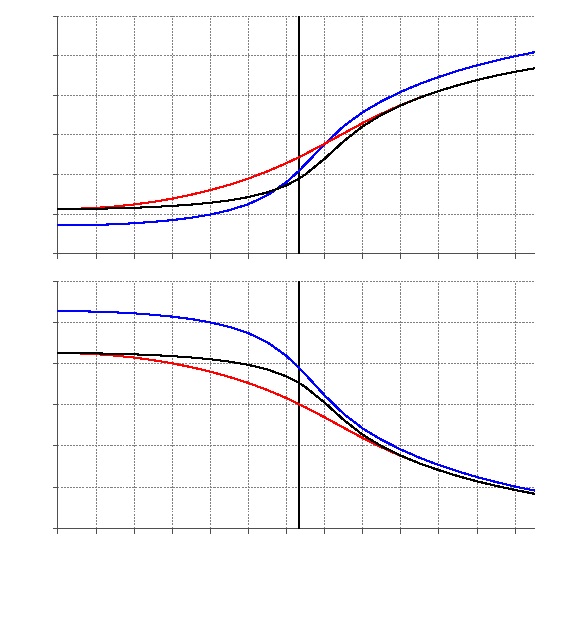
\includegraphics{images/electronicOccupations}}%
    \gplfronttext
  \end{picture}%
\endgroup

  \caption[Probability of finding the system with one charge in an oxygen and the other at the copper and both charges at opposing oxygen sites.]
  {Probability of finding the system with one charge in an oxygen and the other at the copper (top panel) and both charges at opposing oxygen sites (bottom panel) as a fucntion of $\lambda_{ir}$.
  The vertical line marks the relevant $\lambda_{ir}=0.1263$ eV value.}
  \label{fig:electronicOccupations}
\end{figure}

For all three eigenstates the general trend is similar; there is a monotonic increase in the probability of finding one charge in the oxygen and the other in the copper sites while the probability of both charges being the opposing oxygen sites decreases.
This can be interpreted as a partial charge localization in the cluster, although there is still some charge movement \cite{GarciaSaraviaOrtizdeMontellano2013}.

\section{Projection into phonon coordinates}

\begin{figure}[ht]
  \centering
  % GNUPLOT: LaTeX picture with Postscript
\begingroup
  \makeatletter
  \providecommand\color[2][]{%
    \GenericError{(gnuplot) \space\space\space\@spaces}{%
      Package color not loaded in conjunction with
      terminal option `colourtext'%
    }{See the gnuplot documentation for explanation.%
    }{Either use 'blacktext' in gnuplot or load the package
      color.sty in LaTeX.}%
    \renewcommand\color[2][]{}%
  }%
  \providecommand\includegraphics[2][]{%
    \GenericError{(gnuplot) \space\space\space\@spaces}{%
      Package graphicx or graphics not loaded%
    }{See the gnuplot documentation for explanation.%
    }{The gnuplot epslatex terminal needs graphicx.sty or graphics.sty.}%
    \renewcommand\includegraphics[2][]{}%
  }%
  \providecommand\rotatebox[2]{#2}%
  \@ifundefined{ifGPcolor}{%
    \newif\ifGPcolor
    \GPcolortrue
  }{}%
  \@ifundefined{ifGPblacktext}{%
    \newif\ifGPblacktext
    \GPblacktextfalse
  }{}%
  % define a \g@addto@macro without @ in the name:
  \let\gplgaddtomacro\g@addto@macro
  % define empty templates for all commands taking text:
  \gdef\gplbacktext{}%
  \gdef\gplfronttext{}%
  \makeatother
  \ifGPblacktext
    % no textcolor at all
    \def\colorrgb#1{}%
    \def\colorgray#1{}%
  \else
    % gray or color?
    \ifGPcolor
      \def\colorrgb#1{\color[rgb]{#1}}%
      \def\colorgray#1{\color[gray]{#1}}%
      \expandafter\def\csname LTw\endcsname{\color{white}}%
      \expandafter\def\csname LTb\endcsname{\color{black}}%
      \expandafter\def\csname LTa\endcsname{\color{black}}%
      \expandafter\def\csname LT0\endcsname{\color[rgb]{1,0,0}}%
      \expandafter\def\csname LT1\endcsname{\color[rgb]{0,1,0}}%
      \expandafter\def\csname LT2\endcsname{\color[rgb]{0,0,1}}%
      \expandafter\def\csname LT3\endcsname{\color[rgb]{1,0,1}}%
      \expandafter\def\csname LT4\endcsname{\color[rgb]{0,1,1}}%
      \expandafter\def\csname LT5\endcsname{\color[rgb]{1,1,0}}%
      \expandafter\def\csname LT6\endcsname{\color[rgb]{0,0,0}}%
      \expandafter\def\csname LT7\endcsname{\color[rgb]{1,0.3,0}}%
      \expandafter\def\csname LT8\endcsname{\color[rgb]{0.5,0.5,0.5}}%
    \else
      % gray
      \def\colorrgb#1{\color{black}}%
      \def\colorgray#1{\color[gray]{#1}}%
      \expandafter\def\csname LTw\endcsname{\color{white}}%
      \expandafter\def\csname LTb\endcsname{\color{black}}%
      \expandafter\def\csname LTa\endcsname{\color{black}}%
      \expandafter\def\csname LT0\endcsname{\color{black}}%
      \expandafter\def\csname LT1\endcsname{\color{black}}%
      \expandafter\def\csname LT2\endcsname{\color{black}}%
      \expandafter\def\csname LT3\endcsname{\color{black}}%
      \expandafter\def\csname LT4\endcsname{\color{black}}%
      \expandafter\def\csname LT5\endcsname{\color{black}}%
      \expandafter\def\csname LT6\endcsname{\color{black}}%
      \expandafter\def\csname LT7\endcsname{\color{black}}%
      \expandafter\def\csname LT8\endcsname{\color{black}}%
    \fi
  \fi
  \setlength{\unitlength}{0.0500bp}%
  \begin{picture}(7936.00,2834.00)%
    \gplgaddtomacro\gplbacktext{%
      \csname LTb\endcsname%
      \put(-63,879){\makebox(0,0)[r]{\strut{}\scriptsize -0.3}}%
      \put(-63,1124){\makebox(0,0)[r]{\strut{}\scriptsize -0.2}}%
      \put(-63,1369){\makebox(0,0)[r]{\strut{}\scriptsize -0.1}}%
      \put(-63,1615){\makebox(0,0)[r]{\strut{}\scriptsize 0}}%
      \put(-63,1860){\makebox(0,0)[r]{\strut{}\scriptsize 0.1}}%
      \put(-63,2105){\makebox(0,0)[r]{\strut{}\scriptsize 0.2}}%
      \put(-63,2350){\makebox(0,0)[r]{\strut{}\scriptsize 0.3}}%
      \put(218,377){\makebox(0,0){\strut{}\scriptsize -0.4}}%
      \put(764,377){\makebox(0,0){\strut{}\scriptsize -0.2}}%
      \put(1309,377){\makebox(0,0){\strut{}\scriptsize 0}}%
      \put(1854,377){\makebox(0,0){\strut{}\scriptsize 0.2}}%
      \put(2400,377){\makebox(0,0){\strut{}\scriptsize 0.4}}%
      \put(-569,1614){\rotatebox{-270}{\makebox(0,0){\strut{}$u_{R}$ (\AA)}}}%
      \put(1309,91){\makebox(0,0){\strut{}}}%
      \put(794,2720){\makebox(0,0)[l]{\strut{}\scriptsize{$\lambda_{ir} = 0.00$ eV}}}%
    }%
    \gplgaddtomacro\gplfronttext{%
    }%
    \gplgaddtomacro\gplbacktext{%
      \csname LTb\endcsname%
      \put(2836,377){\makebox(0,0){\strut{}\scriptsize -0.4}}%
      \put(3382,377){\makebox(0,0){\strut{}\scriptsize -0.2}}%
      \put(3928,377){\makebox(0,0){\strut{}\scriptsize 0}}%
      \put(4473,377){\makebox(0,0){\strut{}\scriptsize 0.2}}%
      \put(5019,377){\makebox(0,0){\strut{}\scriptsize 0.4}}%
      \put(3278,1614){\rotatebox{-270}{\makebox(0,0){\strut{}}}}%
      \put(3927,47){\makebox(0,0){\strut{}$u_{ir}$ (\AA)}}%
      \put(3412,2720){\makebox(0,0)[l]{\strut{}\scriptsize{$\lambda_{ir} = 0.1263$ eV}}}%
    }%
    \gplgaddtomacro\gplfronttext{%
    }%
    \gplgaddtomacro\gplbacktext{%
      \csname LTb\endcsname%
      \put(5455,377){\makebox(0,0){\strut{}\scriptsize -0.4}}%
      \put(6001,377){\makebox(0,0){\strut{}\scriptsize -0.2}}%
      \put(6546,377){\makebox(0,0){\strut{}\scriptsize 0}}%
      \put(7091,377){\makebox(0,0){\strut{}\scriptsize 0.2}}%
      \put(7637,377){\makebox(0,0){\strut{}\scriptsize 0.4}}%
      \put(5897,1614){\rotatebox{-270}{\makebox(0,0){\strut{}}}}%
      \put(6546,91){\makebox(0,0){\strut{}}}%
      \put(6031,2720){\makebox(0,0)[l]{\strut{}\scriptsize{$\lambda_{ir} = 0.25$ eV}}}%
    }%
    \gplgaddtomacro\gplfronttext{%
    }%
    \gplbacktext
    \put(0,0){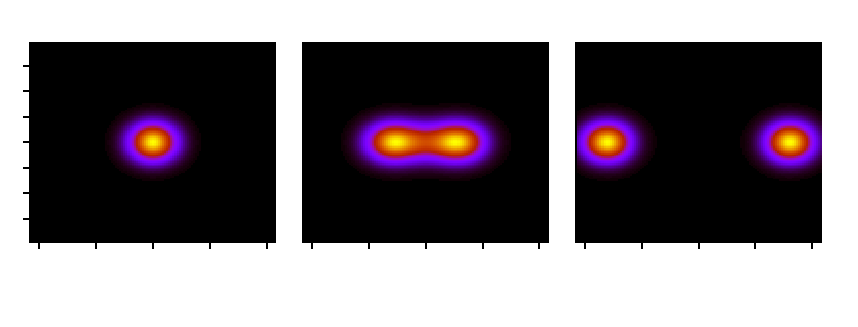
\includegraphics{images/phononProjElectr}}%
    \gplfronttext
  \end{picture}%
\endgroup

  \caption{Electronic state projected into phonon coordinates for three representative electron-lattice coupling ($\lambda_{ir}$) values.}
  \label{fig:phononProjElectr}
\end{figure}

\section{Isotopic shift}

\begin{figure}[ht]
  \centering
  % GNUPLOT: LaTeX picture with Postscript
\begingroup
  \makeatletter
  \providecommand\color[2][]{%
    \GenericError{(gnuplot) \space\space\space\@spaces}{%
      Package color not loaded in conjunction with
      terminal option `colourtext'%
    }{See the gnuplot documentation for explanation.%
    }{Either use 'blacktext' in gnuplot or load the package
      color.sty in LaTeX.}%
    \renewcommand\color[2][]{}%
  }%
  \providecommand\includegraphics[2][]{%
    \GenericError{(gnuplot) \space\space\space\@spaces}{%
      Package graphicx or graphics not loaded%
    }{See the gnuplot documentation for explanation.%
    }{The gnuplot epslatex terminal needs graphicx.sty or graphics.sty.}%
    \renewcommand\includegraphics[2][]{}%
  }%
  \providecommand\rotatebox[2]{#2}%
  \@ifundefined{ifGPcolor}{%
    \newif\ifGPcolor
    \GPcolortrue
  }{}%
  \@ifundefined{ifGPblacktext}{%
    \newif\ifGPblacktext
    \GPblacktextfalse
  }{}%
  % define a \g@addto@macro without @ in the name:
  \let\gplgaddtomacro\g@addto@macro
  % define empty templates for all commands taking text:
  \gdef\gplbacktext{}%
  \gdef\gplfronttext{}%
  \makeatother
  \ifGPblacktext
    % no textcolor at all
    \def\colorrgb#1{}%
    \def\colorgray#1{}%
  \else
    % gray or color?
    \ifGPcolor
      \def\colorrgb#1{\color[rgb]{#1}}%
      \def\colorgray#1{\color[gray]{#1}}%
      \expandafter\def\csname LTw\endcsname{\color{white}}%
      \expandafter\def\csname LTb\endcsname{\color{black}}%
      \expandafter\def\csname LTa\endcsname{\color{black}}%
      \expandafter\def\csname LT0\endcsname{\color[rgb]{1,0,0}}%
      \expandafter\def\csname LT1\endcsname{\color[rgb]{0,1,0}}%
      \expandafter\def\csname LT2\endcsname{\color[rgb]{0,0,1}}%
      \expandafter\def\csname LT3\endcsname{\color[rgb]{1,0,1}}%
      \expandafter\def\csname LT4\endcsname{\color[rgb]{0,1,1}}%
      \expandafter\def\csname LT5\endcsname{\color[rgb]{1,1,0}}%
      \expandafter\def\csname LT6\endcsname{\color[rgb]{0,0,0}}%
      \expandafter\def\csname LT7\endcsname{\color[rgb]{1,0.3,0}}%
      \expandafter\def\csname LT8\endcsname{\color[rgb]{0.5,0.5,0.5}}%
    \else
      % gray
      \def\colorrgb#1{\color{black}}%
      \def\colorgray#1{\color[gray]{#1}}%
      \expandafter\def\csname LTw\endcsname{\color{white}}%
      \expandafter\def\csname LTb\endcsname{\color{black}}%
      \expandafter\def\csname LTa\endcsname{\color{black}}%
      \expandafter\def\csname LT0\endcsname{\color{black}}%
      \expandafter\def\csname LT1\endcsname{\color{black}}%
      \expandafter\def\csname LT2\endcsname{\color{black}}%
      \expandafter\def\csname LT3\endcsname{\color{black}}%
      \expandafter\def\csname LT4\endcsname{\color{black}}%
      \expandafter\def\csname LT5\endcsname{\color{black}}%
      \expandafter\def\csname LT6\endcsname{\color{black}}%
      \expandafter\def\csname LT7\endcsname{\color{black}}%
      \expandafter\def\csname LT8\endcsname{\color{black}}%
    \fi
  \fi
  \setlength{\unitlength}{0.0500bp}%
  \begin{picture}(6802.00,4534.00)%
    \gplgaddtomacro\gplbacktext{%
      \colorrgb{0.31,0.31,0.31}%
      \put(1210,751){\makebox(0,0)[r]{\strut{}\scriptsize -2}}%
      \colorrgb{0.31,0.31,0.31}%
      \put(1210,1191){\makebox(0,0)[r]{\strut{}\scriptsize -1.5}}%
      \colorrgb{0.31,0.31,0.31}%
      \put(1210,1631){\makebox(0,0)[r]{\strut{}\scriptsize -1}}%
      \colorrgb{0.31,0.31,0.31}%
      \put(1210,2070){\makebox(0,0)[r]{\strut{}\scriptsize -0.5}}%
      \colorrgb{0.31,0.31,0.31}%
      \put(1210,2510){\makebox(0,0)[r]{\strut{}\scriptsize 0}}%
      \colorrgb{0.31,0.31,0.31}%
      \put(1210,2950){\makebox(0,0)[r]{\strut{}\scriptsize 0.5}}%
      \colorrgb{0.31,0.31,0.31}%
      \put(1210,3390){\makebox(0,0)[r]{\strut{}\scriptsize 1}}%
      \colorrgb{0.31,0.31,0.31}%
      \put(1210,3829){\makebox(0,0)[r]{\strut{}\scriptsize 1.5}}%
      \colorrgb{0.31,0.31,0.31}%
      \put(1210,4269){\makebox(0,0)[r]{\strut{}\scriptsize 2}}%
      \colorrgb{0.31,0.31,0.31}%
      \put(1389,484){\makebox(0,0){\strut{}\scriptsize 0}}%
      \colorrgb{0.31,0.31,0.31}%
      \put(1790,484){\makebox(0,0){\strut{}\scriptsize 0.02}}%
      \colorrgb{0.31,0.31,0.31}%
      \put(2192,484){\makebox(0,0){\strut{}\scriptsize 0.04}}%
      \colorrgb{0.31,0.31,0.31}%
      \put(2593,484){\makebox(0,0){\strut{}\scriptsize 0.06}}%
      \colorrgb{0.31,0.31,0.31}%
      \put(2994,484){\makebox(0,0){\strut{}\scriptsize 0.08}}%
      \colorrgb{0.31,0.31,0.31}%
      \put(3395,484){\makebox(0,0){\strut{}\scriptsize 0.1}}%
      \colorrgb{0.31,0.31,0.31}%
      \put(3797,484){\makebox(0,0){\strut{}\scriptsize 0.12}}%
      \colorrgb{0.31,0.31,0.31}%
      \put(4198,484){\makebox(0,0){\strut{}\scriptsize 0.14}}%
      \colorrgb{0.31,0.31,0.31}%
      \put(4599,484){\makebox(0,0){\strut{}\scriptsize 0.16}}%
      \colorrgb{0.31,0.31,0.31}%
      \put(5001,484){\makebox(0,0){\strut{}\scriptsize 0.18}}%
      \colorrgb{0.31,0.31,0.31}%
      \put(5402,484){\makebox(0,0){\strut{}\scriptsize 0.2}}%
      \colorrgb{0.31,0.31,0.31}%
      \put(5803,484){\makebox(0,0){\strut{}\scriptsize 0.22}}%
      \colorrgb{0.31,0.31,0.31}%
      \put(6204,484){\makebox(0,0){\strut{}\scriptsize 0.24}}%
      \csname LTb\endcsname%
      \put(176,2510){\rotatebox{-270}{\makebox(0,0){\strut{}$\omega_i$ (cm$^{-1}$)}}}%
      \put(3897,154){\makebox(0,0){\strut{}$\lambda_{ir}$ (eV)}}%
      \put(3997,3988){\makebox(0,0)[l]{\strut{}\scriptsize$\lambda_{ir}=0.1263$}}%
    }%
    \gplgaddtomacro\gplfronttext{%
    }%
    \gplbacktext
    \put(0,0){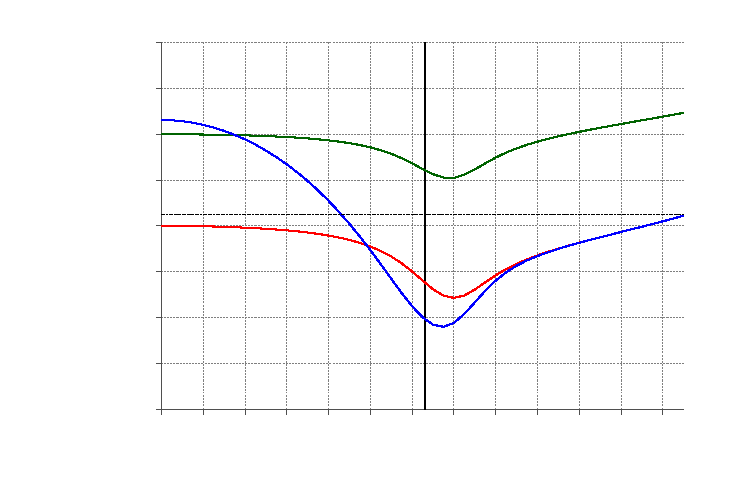
\includegraphics{images/electrIsot}}%
    \gplfronttext
  \end{picture}%
\endgroup

  \caption[Isotopic shift of the electronic excitations as a function of $\lambda_{ir}$.]
  {Isotopic shifts of the electronic excitations as a function of $\lambda_{ir}$. 
    The red line corresponds to an electronic excitation with zero phonons, the blue line with one infrared phonon and the green line with one Raman phonon.
    The vertical line is placed at the relevant value $\lambda_{ir}=0.1263$ eV.}
  \label{fig:electrIsot}
\end{figure}

